\chapter{Вглубь атома}

\epigraph{\emph{... принципиальный вопрос, почему в материальном мире мы снова и снова встречаем повторяющиеся формы и качества}}
{Вернер Гейзенберг}

Математика, используемая в базовых моделях ядерной физики, в целом не очень сложна.
Можно было бы сразу перейти к сути вопроса, как это обычно и делается в книгах по математическим вопросам ядерной физики.
Такой подход имеет свой смысл.
Дело в том, что оформившаяся математическая теория того или иного процесса вполне может быть изложена отдельно от своего физического контекста.
И тем не менее на начальном этапе математику, стоящую за ядерной физикой, не стоит пытаться рассматривать в отрыве от самого ее предмета - атома.
Для полного понимания используемых моделей крайне полезно иметь хотя бы общие представления как об основах ядерной физики, так и о сложном пути, который прошла эта прекрасная наука.

На протяжении всей книги нам не потребуются ни глубокие факты современной ядерной физики, ни продвинутый аппарат квантовой механики.
Для наших целей вполне достаточно будет общих знаний о строении атома и ядерных реакциях.
Без них было бы крайне тяжело понять, почему те или иные задачи ставились перед физиками и математиками Манхэттенского проекта.

В данной главе мы проследим в общих чертах извилистый путь идеи об атоме от туманных философских догадок древности вплоть до современной точки зрения. 
У нас нет цели глубоко погружаться в историко-философские вопросы атомизма.
Мы наметим лишь общий ход его истории как мировоззрения, останавливаясь только на наиболее ярких идеях и открытиях.
В конце главы мы опишем модель атома и процесса ядерного распада, принятые сегодня и не слишком отличающиеся от известных во времена Манхэттенского проекта.
Читатель, знакомый с основами физики атома, может пропустить эту главу и сразу перейти к математической части в гл.~\ref{why_math}.


\section*{Первые идеи}

С древнейших времен не прекращались попытки человека проникнуть в суть материальных объектов, мысленно разбив их на минимально возможные части.
Вообще говоря, это универсальный метод исследования любых сложных объектов - пытаться разложить их на более простые, желательно элементарные части. 
Далее следует следует изучить отдельно каждую часть и то, как они взаимодействуют друг с другом.
Поэтому не столь удивительно, что ученые древности пытались найти и описать некие универсальные первоэлементы, из которых должны состоять все объекты окружающего мира.
История этих попыток насчитывает более двух с половиной тысяч лет.

Начало истории об атоме теряется в древних веках.
Доподлинно неизвестно, когда и кому впервые пришла в голову знаменательная идея о том, что все наблюдаемые в природе объекты при всем многообразии их форм и свойств обязаны состоять из \textit{элементарных} частиц.
Скорее всего это происходило независимо в разное время и в разных культурах.
Наиболее хорошо восстановлен и изучен античный атомизм, но и греки переняли его от более древних цивилизаций Востока, Вавилона и, вероятно, Египта.
Важно, что именно в древней Греции атомизм заиграл всеми красками, глубоко проникая и давая плоды в философии, физике и даже самой математике.

В древности практически одновременно возникли два взгляда на атомарную структуру объектов - философский и математический.
Философский атомизм пытался описать все объекты реального мира как состоящие из некоторых элементарных неделимых частиц, движущихся в абсолютной пустоте.
Математический атомизм носил выраженный прикладной характер, служа вполне конкретной цели - точному вычислению площадей и объемов тел, представляя их в виде совокупности \textit{бесконечно малых} слоев.
Позже мы увидим (см. главу ?????), что это по сути единственный возможный способ определения \textit{меры} (площади или объема) сложного объекта - приблизить его более простыми объектами, мера которых известна.
Именно так определяют меру объектов на плоскости и в пространстве в современной математике.
Оба этих подхода, философский и математический, тесно переплетались, служа постоянными генераторами новых идей, дополняя и подкрепляя друг друга.

Истоки математического атомизма стоит искать у Пифагора и его учеников в VI веке до н.э. 
О тех временах осталось совсем немного достоверных свидетельств.
Вымыслы и легенды практически не отделимы от реальных событий.
Более-менее достоверно известно, что в центр своего учения пифагорейцы ставили целые числа.
Они считали, что все объекты Вселенной должны описываться ими или их отношениями - дробями.
По легенде, эта атомистическая числовая концепция была опровергнута одним из пифагорейцев - Гиппасом, впервые нашедшим несоизмеримые отрезки, то есть отрезки, отношение длин которых не равно никакому отношению двух целых чисел.
Неизвестно, что это были за отрезки - диагональ и сторона квадрата, правильного пятиугольника или что-то еще.
Также неизвестно наказание, которое Гиппас понес за свое открытие - смерть или простое изгнание.   
Так или иначе, атомистическая концепция в целых числах продержалась недолго, но вместе с наследием более древних народов натолкнула на правильные мысли более поздних математиков античности.

Возникновение философского атомизма в его классическом виде связывают с именами двух мыслителей античности - Левкиппа и Демокрита.
Про первого известно совсем немного.
Труды Левкиппа не дошли до нашего времени.
Некоторые историки ставят под сомнение даже само его существование, настолько мало информации о нем осталось.
Демокрит же, несмотря на множество легенд и анекдотичных историй о себе, является вполне реальной исторической фигурой. 
За свой оптимизм и привычку смеяться он был известнен как ``смеющийся философ''.
По одной из легенд, соседи, обеспокоенные постоянными приступами его смеха, вызывали к нему самого Гиппократа, который не выявил у Демокрита опасных отклонений.
По другой легенде, Демокрит ослепил себя, чтобы зрение не мешало мысли. 
Это, впрочем, считается маловероятным.
Скорее всего, зрение Демокрит потерял естественным образом, а прожил он, по разным источикам, от 90 до 109 лет.

Будучи сыном одного из богатейших жителей Абдер - города на севере Греции, Демокрит получил прекрасное образование.
Большую часть юности и наследства он потратил на путешествия, впитывая знания Древнего Египта, Индии, Персии и Вавилона.
По собственному выражению, он ``объездил больше земли, чем кто-либо из современных ... людей, подробнейшим образом исследуя ее''.
Интересно, что за подобные растраты его по закону Абдер ждало наказание.
Однако по легенде, Демокриту удалось склонить судей на свою сторону, зачитав им отрывок одной из книг, написанных во время путешествий.
Судьи сочли подобный труд достойным оправданием и не стали наказывать Демокрита за растрату наследства. 

Демокрит по праву считается одним из основных создателей древнегреческого атомизма в его классическом виде.
Он впервые обобщил имеющиеся древние знания и выдвинул гипотезу о атоме, которая и стала впоследствии фундаментом для всей последующей науки.
Среди всех источников древности, наибольшее влияние на будущие научные интересы Демокрита, по всей видимости, оказали знания Вавилона.
Именно пленные халдеи (представители семитских племен Вавилона) передали ему среди прочего свои соображения об устройстве мира, которые он затем блестяще развил.

В основу учения Демокрита легли следующие утверждения:
\begin{itemize}
    \item Вселенная состоит из \textit{Великой Пустоты} и бесконечного множества \textit{атомов} - неделимых частиц, различных по форме и размеру, но неразрушимых, однородных и непроницаемых.
    \item \textit{Атомы} взаимодействуют друг с другом путем случайных столкновений, являющихся причиной всех остальных движений. 
    \item Все объекты мира состоят из конечного числа \textit{атомов}.
    \item Никакие объекты не возникают из ничего и не исчезают бесследно, только путем комбинации или распада других объектов.
\end{itemize} 
Эти мысли, пока еще чисто философские, стали важной вехой не только философии, но и всей науки в целом.
Несмотря на игнорирование и даже явную критику философии Демокрита признанным тогда авторитетом Платоном, атомизм выдержал испытание временем и в итоге лег в основу всей современной физики и химии.

В свою очередь, идеи математического атомизма, рассорившие адептов крупнейшей античной математической школы Пифагора, послужили хорошей почвой для новых идей как философии, так и в самой математике.
Через некоторое время они были существенно развиты и с успехом использовались Евдоксом, а затем и самим Архимедом.

Арихимед, великий ученый античности, получил прекрасное образование в Александрии - одном из крупнейших научных центров того времени. 
Там он среди прочего изучал труды Демокрита и Евдокса, откуда и узнал об идее атомизма в ее математической и философской интерпретациях.
Фактически только из трудов Архимеда и можно узнать об античном атомизме, так как все, что было до него, по большей части утеряно.
Сам Архимед использовал концепцию математического атомизма в виде значительно усовершенствованной им более ранней \textit{идеи равносоставленности} Евдокса.

\begin{figure}[t!]
   \centering
   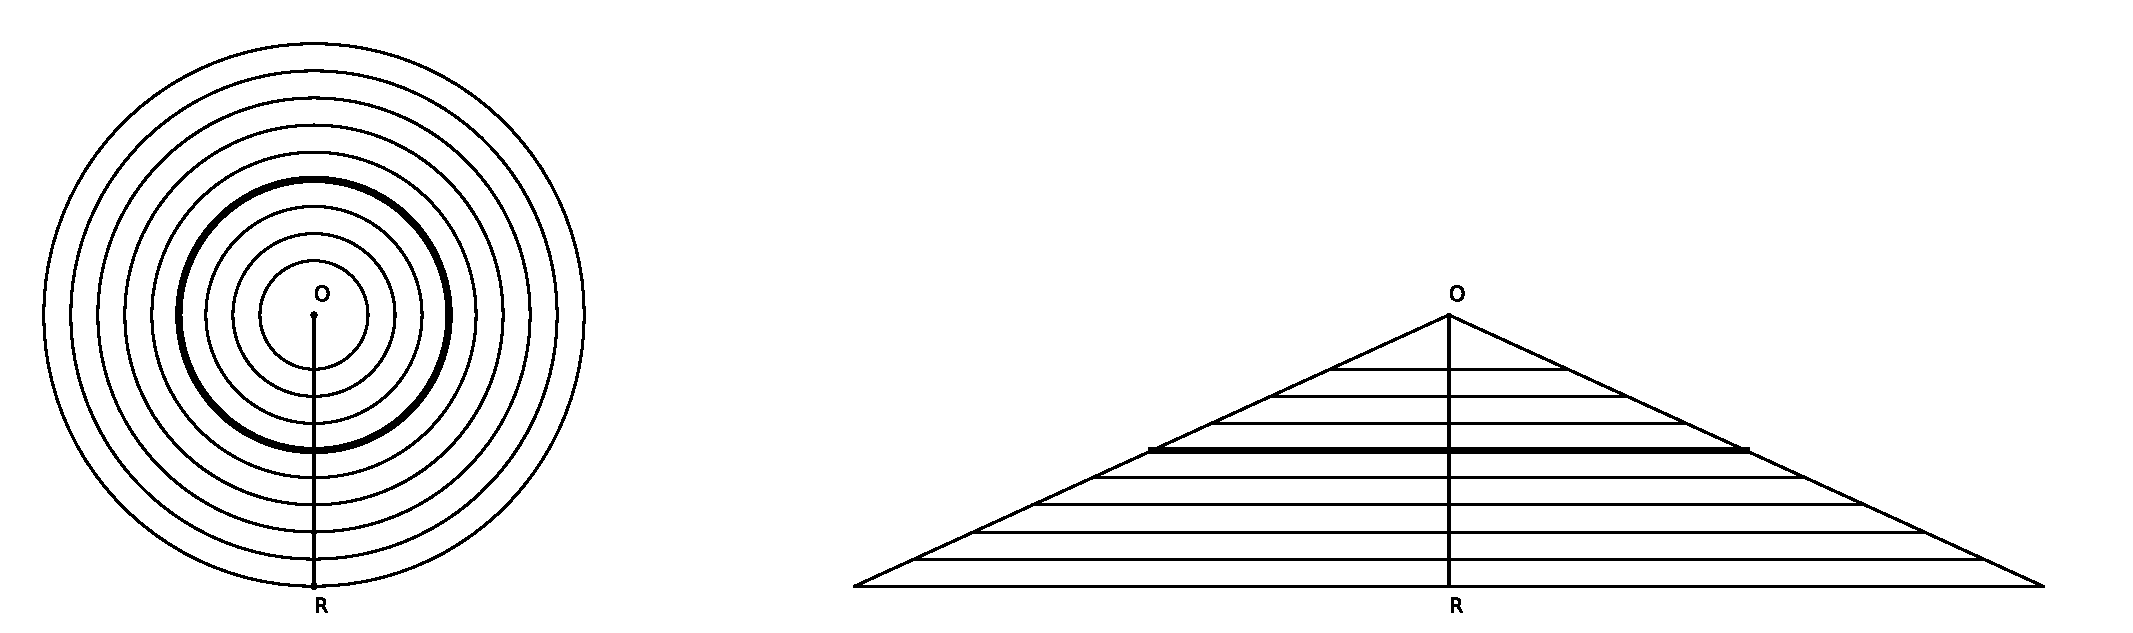
\includegraphics[scale=0.44]{images/archimed_1}
   \caption{Равносоставленность круга и треугольника.}
   \label{fig:archimed_1}
\end{figure}

Идею равносоставленности можно проиллюстрировать на следующем примере (см. рис. \ref{fig:archimed_1}).
Рассмотрим круг радиуса $R$ на плоскости.
Постараемся найти его площадь, зная что длина окружности есть произведение $2\pi$ на ее радиус.
Представим круг состоящим из неделимых объектов - концентрических окружностей с центром в центре круга.
Далее мысленно разрежем круг вдоль вертикального радиуса $OA$ и развернем каждую окружность в отрезок, сохранив ее длину и положение середины на нижнем радиусе $OR$.
В результате получится треугольник с основанием $2\pi R$ и высотой $R$.
По известной формуле, его площадь равна
\begin{equation}\label{eq:ball_square}
S = 2\pi R\cdot\frac{R}{2} = \pi R^2.
\end{equation}
Заметим, что исходный круг и полученный треугольник \textit{равносоставленны}: каждой внутренней окружности круга однозначно соответствует горизонтальный отрезок треугольника, причем той же самой длины.
Так что можно ожидать, что найденное значение \ref{eq:ball_square} равно искомой площади круга, что действительно верно.

К сожалению, принцип равносоставленности в такой интерпретации годится только для отдельных случаев и в целом неверен. 
Несложно придумать, как говорят в математике, \textit{контрпример} рассуждений подобного рода, приводящим к совершенно неверным результатам.
Интересно, что и сам Архимед не относился к этому методу как к строгому, вероятно зная, что он может привести к ошибкам.
Архимед использовал его скорее как способ угадать правильный ответ, который затем тщательно проверял.
И тем не менее, отношение к идее атомизма как конкретному математическому инструменту (пусть и не идеальному) позволило античным ученым заложить основы современного интегрального исчисления, а вместе с ним и значительной части современной математики.

В древние времена и далее в Средневековье и Новое время математический атомизм зарекомендовал себя как крайне эффективный и точный инструмент для самых разных вычислений в любых науках, где только возникали числа. 
Он стал основой для всей последующей математики как науки.
Практически весь аппарат математического анализа, развитого позднее в трудах Ньютона, Лейбница, Кеплера, Лапласа и многих других выдающихся ученых, так или иначе можно считать развитием идей Архимеда и Евдокса.
Даже беглый обзор этих достижений занял бы не одну главу и далеко увел бы нас от основного предмета книги - атома как физического объекта.
Здесь мы должны отвлечься от математического атомизма и вернуться к атомизму философскому, так как именно он дал начало физике атома.


Идеи раннего атомизма, конечно же, были довольно далеки от современного взгляда на вещи.
И тем не менее кажется удивительным то, как далеко удалось продвинуться в своих размышлениях философам древности, не обладавшим серьезными измерительными приборами и сознательно избегавшим экспериментов, доверяя лишь чистой мысли.
Даже те начальные знания, полученные учеными древности практически только силой мысли, имеют прямые параллели с самыми современными взглядами на вещи.
При должной фантазии в философских учениях восточной и греческой философии вполне можно увидеть намеки на современное представление о микромире.
В буддизме, например, с древних времен фактически фигурировал вакуум как материальная среда, в которой мельчайшие частицы непрерывно возникают и исчезают. 
Сегодня подобный взгляд на вещи составляет основу квантовой теории поля, согласно которой так называемые \textit{виртуальные частицы} ведут себя схожим образом. 
Атомы по Демокриту участвовали в непрерывных случайных столкновениях друг с другом, порождая всевозможные движения объектов. 
Последнее весьма похоже на описание броуновского движения, если считать атомы Демокрита современными молекулами.

Античный период в истории характеризуется общим расцветом культуры, искусства, философии и естественных наук.
Активно развивались астрономия, математика, из философии понемногу выделялась физика как самостоятельная экспериментальная наука.
К сожалению, за резким подъемом последовал резкий и продолжительный упадок, грозивший полной или частичной утратой древних знаний.
Не обошла эта участь и философию атомизма.
В период раннего Средневековья он фактически находился под запретом господствующей религии и чуть не был утерян совсем.


\section*{Средневековье}

Атомизм был довольно популярен в античности, но в средние века уступил взглядам Платона и Аристотеля, частично поддерживаемым набирающим силу христианством.
Лишь в X веке к философии Демокрита стали постепенно и осторожно возвращаться.
Примечательно, что происходило это именно в христианских монастырях Англии, Ирландии и Франции.
В то время спорить с доминирущими религиозно-политическими устоями можно было лишь пассивно и обладая достаточным уровнем влияния, то есть по факту быть не только ученым, но в первую очередь и священнослужителем высокого ранга.
Как и в античности, такие авторитеты определялись весьма редким сочетанием хорошей финансовой обеспеченности и тяги к знаниям.

Одними из первых влиятельных покровителей науки в Средневековье стали Герберт Аврилакский и его ученик Фульберт Шартрский.
Герберт был ученым и видным церковным и политическим деятелем.
Он с детства интересовался наукой и получил отличное по тем временам образование, проводя время за изучением достижений арабской и древнегреческой математики, астрономии и философии.
Вместе с этим он сделал блестящую карьеру в церкви, быстро став архиепископом, а затем и папой Сильвестром II.
Используя свое значительное влияние и сохранив приобретенную в юношестве тягу к знаниям, Герберт сыграл выдающуюся роль популяризатора науки в целом и философии атомизма в частности.
Именно благодаря нему монастыри снова стали основными центрами просвещения своего времени.

При жизни Герберта, даже будучи Папой Сильвестром II, неоднократно обвиняли в колдовстве, отступничестве от христианской веры и других грехах, выдумывая красочные легенды на этот счет.
По одной из таких легенд, Герберт с помощью черной магии создал медную голову, умевшую односложно отвечать на все его вопросы и помогавшую ему избегать опасности.
В другом варианте этой легенды, магическую голову вручили ему последователи тайного индийского культа.
Даже за малую часть того, что рассказывали о Герберте обычный человек в то время вполне мог поплатиться жизнью.
Можно только вообразить себе, каким влиянием нужно было обладать, чтобы не только успешно избегать прямого конфликта с недругами, но и продолжать играть роль просветителя в те темные времена.

Многое для развития науки и образования в XI веке сделал французский ученый и теолог Фульберт Шартрский, которого при жизни сравнивали с Сократом.
Будучи епископом, он превратил Шартрский собор в центр преподавания философии, наук и искусств.
Особый акцент делался на математике, что выдает его особую любовь к этой науке.
Философам Шартрской Школы атомизм обязан своим возрождением не в меньшей степени, чем Герберту Аврилакскому.

Благодаря усилиям Герберта, Фульберта и других ученых священнослужителей Средневековья частично утраченные и забытые знания снова становились доступными для изучения и обсуждений.
Науки Востока и античности постепенно возрождались после почти 1000-летнего забвения.
Возвращалась сама культура логических рассуждений, а вместе с ней и истинно научный способ получения новых знаний.

Открыто об идеях Демокрита заговорили лишь еще через 700 лет.
Последней яркой фигурой средневекового атомизма стал католический священник Пьер Гассенди, фактически воскресивший его на рубеже Средневековья и Нового времени.
Гассенди был во многом выдающейся личностью своего времени. 
Аббат и профессор теологии в юношестве и профессор математики впоследствии, помимо богословия активно интересовался физикой, астрономией и математикой. 
Десятиления упорного труда ушли у него на восстановление забытых или запрещенных ранее трудов древнегреческих философов. 
Принятая Гассенди точка зрения на атомизм во многом повторяла учение Демокрита о пустом пространстве и существующих в нем неделимых элементах материи - атомах. 
Он добавил к классическому атомизму один очень существенный элемент - в 1647 году впервые ввел в науку понятие \textit{молекулы} как соединения отдельных атомов. 
Гассенди пришел к верному выводу, что все тела состоят из молекул, и именно молекулы определяют их основные свойства.

Идея о молекулярном строении тел не была далеко развита самим Гассенди, но высоко ценилась выдающимися учеными Нового времени - Бойлем и Ньютоном.
Именно Бойль под влиянием молекулярной теории Гассенди впоследствии развил свою теорию, объясняющую физические и химические явления в газах.    

Распространение учения об атоме в Средневековье во многом обязано отдельным выдающимся личностям, пытавшимся примирить его с религией.
Спорить с господствующей более тысячи лет догмой могли только влиятельные религиозные и политические фигуры, но даже они довольно сильно рисковали.
Хотя нет прямых свидетельств жестокого преследования атомизма со стороны инквизиции, учение это было крайне непопулярно.
Его приверженцам зачастую приходилось приносить долгие официальные извинения.

Ценность эпохи Средневековья для атомизма заключается не столько в конкретных достижениях, сколько в самом факте того, что он не был утерян совсем и продолжил свое развитие далее, в Новое время.


\section*{Новое время}

Конец эпохи Средневековья характеризовался постепенным снятием религиозных запретов на целые области древних и новых наук. 
Это позволило кардинально переосмыслить как имеющиеся знания, так и сам метод получения новых.
Стало ясно, что внимания достойны лишь те факты и наблюдения, которые можно повторить и проверить.
Сила авторитетов древности начала уступать силе объективных знаний и основному способу их получения - научному методу.
Новая методология научного исследования, сформулированная в XVI-XVII веке Френсисом Бэконом, опиралась на следующий принцип: \textit{источником знания и критерием его истинности является только опыт, который можно повторять необходимое число раз}.

\textit{Научный метод} Бэкона устанавливал следующий процесс получения новых фактов об устройстве мира: 
\begin{itemize}
    \item наблюдение,
    \item формулировка гипотез,
    \item проведение необходимых экспериментов для их подтверждения или опровержения,
    \item проверка воспроизводимости всех полученных результатов.
\end{itemize}
Сейчас подобный подход к исследованиям кажется простым и естественным, но в то время это была настоящая революция.
До этого считалось, что ответы на все вопросы можно найти у Аристотеля.
Научный подход исключал субъективность и позволял каждому желающему убедиться в справедливости выдвинутых кем-либо теорий.
Теперь каждый мог привнести в науку что-то свое.
Нужно было лишь поставить соответствующий эксперимент, выдвинуть гипотезы и подтвердить свои догадки.

Новый подход к знаниям коснулся всех научных идей древности и в первую очередь самого атомизма.
К счастью, Средневековье не только сохранило его как систему взглядов, но и привнесло новое важное понятие молекулы, которое стало ключевым для дальнейшего понимания устройства мира. 
Теперь это понятие предстояло уточнять и строить на его основе не только качественные догадки, но и делать количественные предсказания.
Новые правила научной игры подходили для этого как нельзя лучше.
Очень скоро из собрания чисто философских идей атомизму предстояло стать прочной основой для всей современной физики и химии.

Первый шаг на этом пути был сделан ирландским ученым и богословом Робертом Бойлем.
Получив в Европе прекрасное образование, богатым наследником он вернулся в родную Ирландию, где полностью посвятил себя науке.
Бойль был не только талантливым экспериментатором, но и одним из первых физиков-теоретиков.
Вдохновившись идеями античных ученых и молекулярной гипотезой Гассенди, он смог существенно продвинуться в вопросах строения вещества. Бойль получил, по сути, первое существенное доказательство существования атомов и молекул.
А именно, опираясь на гипотезу о молекулярном строении вещества, Бойль в 1662 году впервые установил строгое математическое соотношение между объемом некоторого газа $p$ и его давлением $V$:

\begin{equation}\label{eq:boil}
pV = c.
\end{equation}

При всей своей простоте эта формула была уже не просто абстрактной философской идеей.
Она позволяла делать как качественные, так и строгие количественные предсказания.
Например, из нее следовало, что при сжатии объема с газом, давление в нем возрастает.
При этом можно посчитать, во сколько именно возрастает давление.
Более того, формула Бойля находилась в прекрасном соответствии с предположением об атомно-молекулярном строении вещества.
Действительно, если в данном ограниченном элементе объема находятся хаотически движущиеся частица газа, то при уменьшении объема давление, вызванное их соударениями со стенкой, будет возрастать.

Формула (\ref{eq:boil}) служила довольно убедительным доводом в пользу существования атомов и молекул.
Другим его значительным вкладом в науку было введение понятия \textit{химического элемента} — мальчайшей составной части простых (одноэлементных) веществ, и входящей в состав сложных.
В своих взглядах на строение веществ Бойль был уже очень близок к современному взгляду на вещи. 

Несколько позднее, в 1676 году французкий ученый Эдм Мариотт подтвердил формулу (\ref{eq:boil}), уточнив, что оно справедливо только при постоянной температуре.
Более точная формула с учетом температуры может быть записана в виде

\begin{equation}\label{eq:boil-mariott}
pV = cT
\end{equation}
с некоторой новой постоянной $c$. 
Из этого соотношения уже видно, что при повышении температуры должен возрастать объем, либо давление, и опять, эти процессы полностью описываются им количественно.
И опять, можно догадаться, что именно хаотическое движение молекул в газе ведет к увеличению его объема, давления, либо температуры.
Замечено это было позднее.
Наконец, и эта формула была уточнена до \textit{уравнения состояния идеального газа} (формула Клапейрона - Менделеева):

\begin{equation}\label{eq:klap-mendeleev}
pV = nRT.
\end{equation}
Здесь уже нет неизвестных констант.
Четкий физический смысл имеет каждая входящая в нее величина.
Эта формула связывает макроскопические характеристики газа - давление, объем и температуру с микроскопической характеристикой - количеством молекул $n$ в одном моле газа, через универсальную газовую постоянную $R$.
Важно понимать, что несмотря на отсутствие неопределенностей, формула (\ref{eq:klap-mendeleev}) тоже имеет свои границы применения.

В истории открытия формулы Бойля - Мариотта - Клапейрона - Менделеева хорошо прослеживается один очень важный принцип.
Каждая из формул (\ref{eq:boil}), (\ref{eq:boil-mariott}), (\ref{eq:klap-mendeleev}) справедлива в своих предположениях и не отменяет, а уточняет предыдущую.
Таким образом, в математической записи законов природы потенциально заложено их возможное обобщение в будущем.
По этой же причине основные уравнения квантовой механики при некоторых условиях могут быть сведены к уравнениям классической физики, а механика теории относительности Эйнштейна является не опровержением, а расширением классической механики Ньютона. 
Это очень важное свойство математических моделей.
Оно говорит о том, что даже математическое описание некоторого явления, удовлетворительно строгое в данный момент, вполне может оказаться неполным в последствии.
И это отнюдь не помешает пользоваться им сейчас и уточнить его в будущем, опираясь на новые наблюдения.

Идея молекулярного строения вещества была далее существенно развита в трудах выдающегося русского ученого М.В. Ломоносова в середине XVIII века.
Ломоносову среди прочего удалось объяснить агрегатные состояния веществ и тепловые эффекты, отвергнув господствующую теорию о теплороде - специальной субстанции, порождающей тепло.
Он пришел к заключению, что молекулы должны находиться в непрерывном движении, что и определяет тепловое состояние тел.
Как он писал, ``теплота состоит в движении материи, которое движение хотя и не всегда чувствительно, однако подлинно в теплых телах есть'' что, таким образом, устраняет ``смутные домыслы о некоторой бродячей, беззаконно скитающейся теплотворной материи''.
Свою теорию ученый подтвердил математическими расчетами и рядом блестящих для того времени экспериментов.

Молекулярно-кинетическая теория Ломоносова подвергалась жесткой критике, но в итоге стала общепризнанной вехой в атомизме.
Тем не менее, Ломоносов ошибся в ряде моментов.
Он представял молекулы шарообразными, причем тепло вырабатывалось путем их вращения, а при колебательном движении, по его мнению, тела должны были разрушаться. 
Ломоносов также не допускал, что молекулы могут соударяться друг с другом, только соприкасаться.
Эти неточности, ликвидированные впоследствии другими учеными, не говорят об ошибочности нучного метода, а скорее демонстрируют его в действии.
По словам самого ученого, ``из наблюдений устанавливать теорию, через теорию исправлять наблюдения есть лучший всех способ к отысканию правды''.
Ломоносову для описания явления распространения тепла вполне хватило правильных предположений, прекрасно подтвердившихся экспериментом.
Неверные гипотезы не помешали общим верным выводам, и были исправлены в дальнейшем, когда в этом возникла необходимость.

Следующие открытия в учении об атоме соединили атомизм с молодой наукой химией и фактически определили ее современный облик.
Они связаны с именами Джона Дальтона и Антуана Лавуазье.
Оба были выдающимися учеными своего времени.

Антуан Лавуазье был сыном состоятельного парижского адвоката. 
Параллельно с изучением юриспруденции в университете, как того хотел его отец, Лавуазье самостоятельно занимался естественными науками, чувствуя в этом свое истинное призвание.
Уже в 25 лет за свои блестящие достижения он был избран сначала адъюнктом Французской Академии наук, а впоследствии и ее действительным членом и директором.
Он внес значительный вклад в не только в химию, но также физику, физиологию и даже гуманитарные науки.

В атомизме достижения Лавуазье связаны развитием введенного Бойлем понятия \textit{элементарного тела} как химически не разложимого вещества.
Идеи Лавуазье значительным образом способствовали открытию впоследствии стехиометрических законов, то есть правил, которым подчиняются массы и объемы реагирующих веществ.
Его эксперименты были беспрецедентно точны и тщательно подготовлены.
Все это способствовало окончательному внедрению идей атомно - молекулярного строения вещества в новую тогда еще науку химию.
Именно использование понятий атома и молекулы позволяло просто и ясно объяснять химические наблюдения, что несомненно говорило в пользу их истинности.

Хотя Лавуазье не имел недостатка в средствах, личное финансовое благополучие интересовало его в гораздо меньшей степени, нежели возможность сделать новое открытие. 
Большие деньги, получаемые на государственной службе, Лавуазье тратил на эксперименты.
К сожалению, именно занимаемая им должность сборщика налогов стала для него роковой.
Ни выдающиеся заслуги перед Францией, ни непререкаемый авторитет в науке, не уберегли Лавуазье от казни по обвинению в государственной измене во время Французской революции.
Просьба Лавуазье об отсрочке своей казни на несколько дней для публикации своих последних работ была отклонена.

О преданности Лавуазье науке можно судить по следующей истории о нем.
Его волновал популярный в то время вопрос, умирает ли голова сразу после отсечения, либо живет еще какое-то время.
Накануне своей казни ученый придумал опыт, позволяющий это определить.
Согласно его задумке, в случае жизни после отсечения голова могла бы подать знак, моргнув одним глазом.  
Понимая, что проверить результаты этого опыта ему уже не удастся, он попросил это сделать палача. 
Палач оценил идею Лавуазье, но тут же заверил, что в этом эксперименте нет никакой необходимости, так как в случае мгновенной смерти казненных ему бы не приходилось время от времени менять обкусанные по краям корзины для голов.

Биограф Лавуазье, выдающийся математик Лагранж писал: ``Всего мгновение потребовалось, чтобы отрубить голову, замену которой невозможно найти и за сотни лет''.

Другой знаковой фигурой химического атомизма Нового времени был Джон Дальтон, сделавший значительный вклад в молекулярную теорию строения вещества.
За свою жизнь Дальтон совершил множество открытий, включая открытие названной его именем болезни, которой страдал сам.
Наиболее замечательными были его достижения в атомно-молекулярной теории.
С его именем, наряду с Лавуазье, связывают становление  современнойхимии как науки.

Дальтон справедливо считал, что атомы участвующих в химических превращениях веществ при химических раекциях не распадаются на части и не создаются, а лишь перераспределяются. 
Таким образом, впервые возникла идея об атоме как \textit{химически неделимом} элементе мироздания, участвующем в любом превращении веществ в природе.
В серии блестящих опытов в начале XIX века Дальтон подтвердил свою теорию.
Он обнаружил, что
\begin{itemize}
    \item давление смеси газов равно сумме давлений каждого газа в отдельности - закон парциальных давлений смесей газов,
    \item растворимость газа в жидкости пропорциональна его парциальному давлению - закон растворимости газов в жидкостях,
    \item закон равномерного расширения газов при нагревании,
    \item если два химических элемента образуют между собой несколько соединений, то отношения масс атомов одного элемента к массам атомов другого элемента между собой соотносятся как целые числа - закон кратных отношений.
\end{itemize}
Эти открытия прекрасно объяснялись атомной гипотезой строения вещества.
Так атомизм античности наконец начал обретать прочный экспериментальный фундамент.

Дальтон не остановился на указанных открытиях и сделал еще один большой шаг по направлению к современным представлениям об атоме.
Он обратил внимание на исключительную роль массы атома в химических превращениях веществ.
Дальтон впервые составил таблицу относительных атомных весов.
Таблица была очень неточна и неоднократно менялась им впоследствии.
Гораздо более точные таблицы были получены впоследствии Авогадро и Берцеллиусом (см. таблицу \ref{tab:atom_mass}).

\begin{table}
\label{tab:atom_mass}
    \begin{center}
        \begin{tabular}{|p{3cm}|p{2cm}|p{2cm}|p{2.2cm}|p{2cm}|}
            \hline
            \multirow{2}{}{Химический элемент} & \multicolumn{4}{|c|}{Относительная атомная масса} \\
            & Дальтон & Авогадро & Берцелиус & Соврем. \\
            \hline
            H & 1 & - & 1 & 1.01 \\
            C & 5.4 & 12.08 & 12.25 & 12.01 \\
            N & 5 & 13.97 & 14.19 & 14.01 \\
            O & 7 & 16.1 & 16.03 & 16.00 \\
            Ag & 10 & 216 & 216.61 & 107.87 \\
            \hline
        \end{tabular}
    \end{center}
\caption{Фрагмент таблицы атомных масс (1 а.е.м.\approx $1.661\cdot 10^{-27}$ кг).}
\end{table}

Новое время стало стало настоящим расцветом для науки.
Идеология ``идея - эксперимент - теория'' быстро прижилась в самых разных областях знаний, давая поразительные результаты.
Лаконично вписались в эту концепцию и математические методы.
Стало ясно, что законы природы должны выражаться в строгих формулах, дающих не только общее описание явления, но и возможность точных предсказаний.
Теперь можно было не только рассуждать об устройстве мира, но и применять эти знания на практике.
Это было серьезным прорывом.

Последующие открытия Нового времени, связанные с понятиями атома и молекулы, были сделаны прежде всего в физической химии. 
Они связаны с именами таких выдающихся ученых как Пруст, Авогадро, Берцеллиус, Бутлеров и Менделеев.
Описание их достижений увело бы нас от основного предмета книги - атома, в сторону химии.
Вместо этого перейдем к открытиям физики начала XX века, ставшим решающими для понимания тайн атома.


\section*{Время новой физики}

---------

Броун


\section*{Строение атома}

Итак, что же такое атом? К настоящему времени известно следующее.
Атом - микроскопическая частица вещества, состоящая из тяжелого ядра, окруженного легкими (по сравнению с ядром) электронами.
Ядро состоит из нуклонов: протонов и нейтронов.
Сами по себе нуклоны в свою очередь состоят из еще более мелких субатомных частиц: глюонов, квакров и антикварков.
Эти частицы интересны в первую очередь тем, что наряду с электронами, вполне могут оказаться действительно \textit{элементарными} - далее неделимыми на более мелкие еще неизвестные науке частицы.

Число протонов в ядре $Z$ называется \textit{зарядовым числом} или \textit{атомным номером}.
Оно однозначно определяет тип химического элемента и его место в периодической таблице элементов. 
Число нейтронов $N$ в ядре не влияет на химические свойства атома и может не совпадать с числов протонов.
Для одного и того же элемента с разным числом нейтронов говорят о его \textit{изотопах}.
Полное количество $A = N + Z$ протонов и нейтронов называют \textit{массовым числом} атома.

\begin{figure}[t!]
   \centering
   \includegraphics[scale=0.4]{images/atom_1}
   \caption{Строение атома гелия: два протона и нейтрона в ядре и два электрона, ``размазанные'' около ядра в облаке формы шарового слоя. Наболее вероятное местонахождение электронов - пунктирная сфера, но точно локализовать электрон в пространстве невозможно.}
   \label{fig:atom_1}
\end{figure}

На рис. \ref{fig:atom_1} изображен атом гелия, имеющего два протона и нейтрона в ядре и два электрона на некотором расстоянии от центра.
Рисунок довольно схематичен, так как в реальности электроны располагаются на очень большом по сравнению с ядром расстоянии от него.
Строение ядра атома гелия, как и любого другого элемента, в целом довольно просто: протоны и нейтроны упакованы в ядре довольно плотно, находясь практически в непосредственной близости друг о друга.
Таким образом, ядро атома представляет собой весьма плотную упаковку из нуклонов.

На значительном расстоянии от ядра находятся электроны.
Число электронов в атоме совпадает с числом протонов $Z$, что гарантирует его электронейтральность.

\subsubsection*{Размеры}

Линейные размеры атома определить достаточно сложно из-за неопределенности положения его электронов в пространстве.
О размерах атома принято судить либо по наиболее вероятной удаленности его электронов от ядра, либо по расстоянию между ядрами двух одинаковых атомов в молекуле простого вещества.
В любом случае они очень малы - от $31\cdot 10^{-12}$ (атом гелия) до $225\cdot 10^{-12}$ (атом цезия) метра.
Порядком размера атома принято считать величину $1\mbox{\normalfont\AA} = 10^{-10}$ м (ангстрем).

Протон имеет размеры порядка $10^{-15}$ метра, а все атомное ядро - $10^{-14}$ метра.
Таким образом, ядро в сотни-тысячи раз меньше, чем весь атом.
В связи с этими числами обычно приводят следующий пример: если ядро увеличить до размеров футбольного шара, то весь атом увеличится до размеров стадиона.

Относительно размеров электрона даже в настоящее время известно очень немногое.
Последние попытки его определения показали, что оно не превосходит $10^{-20}$ метра.
Электрон принято считать \textit{фундаментальной элементарной частицей}, то есть такой, которую пока не удалось разложить на составные частицы и определить ее размер.

Если учесть, что наиболее вероятные места пребывания электронов сконцентрированы около поверхностей типа сферы на рис. \ref{fig:atom_1} - фигур нулевого объема в пространстве, то электронному облаку можно не приписывать сколько-нибудь существенного объема.
Если при это учать неимоверно малые размеры атомных ядер, которые также состоят из более мелких элементарных частиц, то получается, что мы живем в практически пустом пространстве.

\subsubsection*{Орбитали}

Главный и наиболее сложный для понимания факт об электронах состоит в том, что их точное местоположение в пространстве указать невозможно.
Они как бы размазаны в пространстве около ядра, одновременно находясь в различных его областях.

Принято говорить, что электроны образуют вокруг ядра \textit{электронное облако} (см. рис. (\ref{fig:atom_1})).
Это довольно нетривиальное понятие.
Во-первых, это не облако из электронов, а нечто более сложное.
Оно представляет собой \textit{плотность вероятности} электрона быть обнаруженным в данной точке пространства (см. главу .....).
Чем выше плотность (более темные области на рис. (\ref{fig:atom_1})), тем больше вероятность обнаружить электрон в этом месте.

Интересно отметить, что в вероятность данном случае отражает не наше субъективное незнание о местонахождении электрона, а объективный факт: положение электрона в простнастве точно определить невозможно в принципе.
И это никак не зависит от наших технических возможностей. 
Например, подбрасывая монетку, мы тоже не знаем, какой стороной она упадет и говорим лишь о вероятности ее выпадения, например, орлом.
Но в этом случае мы принципиально могли бы точно предсказать результат броска, если бы знали силу и скорость броска и точно описали бы турбулентные движения воздуха около монетки.
С электронами все иначе.
Мы в принципе лишены возможности обладания \textit{скрытой информацией}, которая в итоге позволила бы точно определить местонахождение электрона.
Оказывается, так устроен мир, и ничего с этим не поделаешь. 

Откуда же можно найти хотя бы вероятность нахождения электрона в заданной области пространства?
Оказывается, она может быть найдена точно как решение уравнения Шреддингера
\begin{equation}\label{eq:schroedinger_1}
\nabla\psi + \frac{2m}{\hbar^2}(E - U)\psi = 0.
\end{equation}
Не вдаваясь в технические детали, скажем, что уравнение (\ref{eq:schroedinger_1}) дает искомую плотность вероятности обнаружения электрона в точке $x$ как квадрат модуля функции-решения $|\psi(x)|^2$.



Локализация в пространстве - орбитали


Поверхность в пространстве вокруг ядра, где плотность вероятности максимальна, называют \textit{орбиталью}.
Таким образом, не совсем правильно думать, что электроны именно вращаются вокруг ядра строго по орбиталям, как движутся по своим орбитам планеты солнечной системы.
Более того, само понятие движения электрона в данном случае весьма условно.
Электрон как бы находится во всех местах одновременно, но в некоторых с большей вероятностью. 
В первом приближении действительно можно представлять себе механическое движение электрона по своей орбитали, и в ряде случаях такая точка зрения не приведет к ошибкам.
Но в целом важно понимать, что орбиталь - лишь наиболее вероятное, но не обязательно точное местонахождение электрона в пространстве.

В простейшем слу


О конкретной траектории движения электрона по орбитали речи идти не может.




\subsubsection*{Масса}

\subsubsection*{Заряд}

\subsubsection*{Стабильность и распад}

Простейшим из атомов является атом водорода, обладающий минимальным числом протонов - одним.
Число нейтронов в атоме водорода может быть от нуля до семи, но с ростом их числа ядро становится нестабильным и быстро спонтанно распадается.
Так, у трития - изотопа водорода с тремя протонами, период полураспада составляет около 12 лет, а у квадия с четырьмя протонами - всего $1.4\cdot 10^{−22}$ секунды.
Это же верно для любых атомов.
Нейтроны необходимы, чтобы стабилизировать пытающиеся разлететься протоны, но с ростом их числа атом все-таки теряет стабильность (см. рис. \ref{fig:atom_stability}).


\begin{figure}[t!]
   \centering
   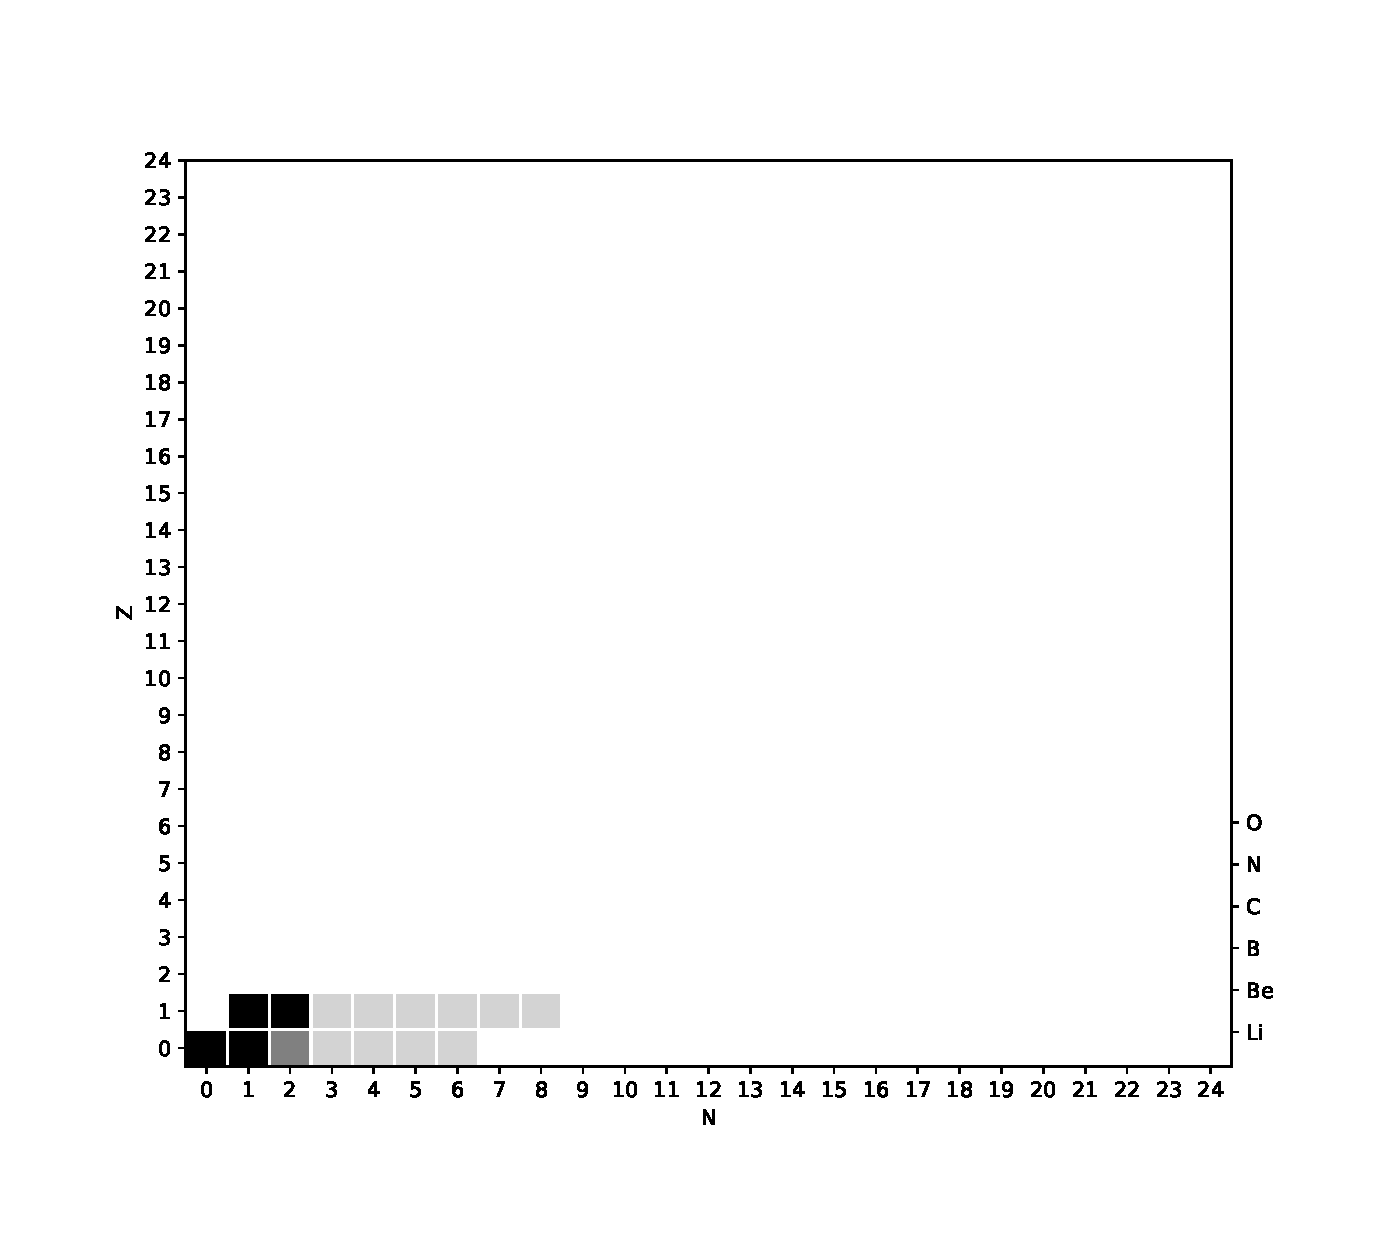
\includegraphics[scale=0.4]{images/atom_stability}
   \caption{Фрагмент диаграммы стабильности атомов химических элементов в зависимости от числа протонов и нейтронов в ядре. Темные клетки - стабильные атомы, светлые - относительно стабильные атомы, живущие от часов до миллиардов лет, пустые - нестабильные атомы, живущие не более малых долей секунд.}
   \label{fig:atom_stability}
\end{figure}




Электроны и протоны являются носителями электрического заряда, нейтроны электрически нейтральны. 
Электроны отрицательно заряжены, протоны - положительно, причем заряд электрона равен заряду протона, а числа электронов и протонов в атоме равны, так что атом оказывается электронейтральным в целом.
Бывает, что атом теряет или приобретает электроны, приобретая таким образом заряд и новое название - ион.
Здесь нас будут интересовать только атомы, не имеющие заряда.

При массе атома от $1.7\cdot 10^{-27}$ кг (атом Водорода-1) до $209.6\cdot 10^{-27}$ кг (атом свинца-208) масса одного электрона составляет всего $9.1\cdot 10^{-31}$ кг.
То есть в ядре сконцентрировано более $99.9\%$ всей массы атома.
Интересно, что кварки, из которых состоят протон, дают менее $2\%$ его массы, основная же часть массы протона приходится на виртуальные частицы.
Нам далее не потребуются столь глубокие субатомные понятия, как кварки и виртуальные частицы. 
Многие из них были открыты и изучены уже после Манхэттенского проекта и никак на него не повлияли. 


\section*{Цепные реакции}

Химические превращения одних веществ в другие происходят только путем перегруппировки атомов между их молекулами.
В процессе химической реакции молекулы исходных веществ отдают или принимают атомы, в результате образуя молекулы новых веществ. 
Сами атомы при этом остаются неизменными.
В этом смысле атом действительно является \textit{наименьшим} носителем химических свойств данного вещества, как и думали древние.

Таким образом, одних простых химических реакций недостаточно, чтобы решить главную задачу алхимии - заставить атомы одного вещества стать атомами другого.
Для того чтобы атомы одного вещества превратились в атомы другого, необходимо более грубое физическое вмешательство - ядерные реакции, в процессе которых ядра атомов взаимодействуют друг с другом или с элементарными частицами.
В результате ядерных реакций тяжелые атомы могут распадаться в более легкие (реакции деления), либо соединяться в еще более тяжелые (реакции синтеза).
Оба этих типа реакций происходят с выделением огромного количества тепла и радиации, что и послужило главной причиной для использования их в военных целях.




------------------------ IDEAS ------------------------ 

По словам Эйнштейна, ``воображение важнее знания, так как знание ограничено''.
В XX веке теории об атоме предстояло пережить... что даже воображение не всегда справлялось...


Атом вполне может приобретать или терять электроны, получая таким образом заряд и становясь \textit{ионом}.
Порцессы ионизации в ядерных реакциях нас не 



атомы - интуиция еще со времен древних греков, но дальше - перерыв почти на x000 лет связанный с тем, что увидеть объект своих измышлений уже не возможно.
прорыв - с появлением соответсвующих средств измерений, но тут ученых ждал очень большой сбрприз
до этого схема научных открытий в большинстве своем состояла в следующем - смотрели, измеряли, придумывали теорию основнную на уже известных аналогиях, потом совершенствовали приборы, и снова смотрели и придумывали анлогию и т.п.
в атомной физике известных аналогий не нашлось. Наблюдения зачастую в корне противоречили известным фактам о макромире. Любая попытка смотреть на макро-аналогии заканчивалась появлением множества противоречий теории с экспериментом и в конце концов полным провалом 


физика - ранее умение делать открытия зависело от того, насколько наблюдателен был ученый, насколько хорошо он умел проводить параллели между уже известными ялениями и только изучаемыми.
Движения огромных небесных тел описывалось исходя из аналогичных движений, которые можно было повторять в удобном масштабе в своей алборатории и т.п. [еще примеры]
Новая физика потребовала от ученых вообразить нечто не имевшее аналогов с ранее изученным в принципе. 
Это восхищало даже далеких от физики современников.
В математике такие штуки привыкли проворачивать довольно давно. 
Стефан Банах, один из создателей современной математики в ее [современном] виде, говорил "Хорошие математики видят аналогии, лучшие могут видеть аналигии между аналогиями". Сам он, безусловно, был одним из лучших.

 
слова "теория относительности", "квантовая механика" носились в воздухе. Их можно было слышать  понимающих и истолковыва

----------------------------



https://ru.wikipedia.org/wiki/%D0%AD%D0%BB%D0%B5%D0%BA%D1%82%D1%80%D0%BE%D0%BD%D0%BD%D0%B0%D1%8F_%D0%BF%D0%BB%D0%BE%D1%82%D0%BD%D0%BE%D1%81%D1%82%D1%8C
{
В качестве модели состояния электрона в атоме, в квантовой механике принято представление об электронном облаке, плотность соответствующих участков которого пропорциональна вероятности нахождения там электрона.

Электронное облако часто изображают в виде граничной поверхности. При этом обозначение электронной области при помощи точек опускают. Пространство вокруг ядра, в котором наиболее вероятно пребывание электрона, называют атомной орбиталью (смысл которого вытекает из волнового уравнения Шрёдингера).

Применяются графические изображения распределения электронной плотности относительно ядра.

Кривая радиального распределения вероятности показывает, что электрон находится в тонком концентрическом шаровом слое радиуса r толщины dr вокруг ядра атома водорода[1].

Проекция максимума кривой соответствует боровскому радиусу alpha_0=0,53 A_with_circle.

Во многих случаях для решения уравнения Шрёдингера используют различные приближения. Вероятностную (статистическую) интерпретацию волновой функции разработал Макс Борн. В 1954 году М.Борн удостоен Нобелевской премии по физике с формулировкой «За фундаментальные исследования в области квантовой механики, особенно, за статистическую интерпретацию волновой функции.»
}

https://ru.wikipedia.org/wiki/%D0%A1%D1%82%D0%B0%D1%82%D0%B8%D1%81%D1%82%D0%B8%D1%87%D0%B5%D1%81%D0%BA%D0%B0%D1%8F_%D0%B8%D0%BD%D1%82%D0%B5%D1%80%D0%BF%D1%80%D0%B5%D1%82%D0%B0%D1%86%D0%B8%D1%8F_%D0%B2%D0%BE%D0%BB%D0%BD%D0%BE%D0%B2%D0%BE%D0%B9_%D1%84%D1%83%D0%BD%D0%BA%D1%86%D0%B8%D0%B8
{
М. Борн вспоминал:
Он (Шрёдингер) рассматривал электрон не как частицу, но как некоторое распределение плотности, которое давалось квадратом его волновой функции |ψ|².

Он считал, что следует полностью отказаться от идеи частиц и квантовых скачков, и никогда не сомневался в правильности этого убеждения. Я, напротив, имел возможность каждодневно убеждаться в плодотворности концепции частиц, наблюдая за блестящими опытами Франка по атомным и молекулярным столкновениям, и был убеждён, что частицы не могут быть упразднены. Следовало найти путь к объединению частиц и волн. Я видел связующее звено в идее вероятности…
}


Французские академики рассказали мне, что Антуан Лавуазье был гильотинирован как "генеральный фермер" — член Королевского колхоза, собиравшего налоги с привозивших в Париж кур крестьян. Перед казнью Лавуазье просил палача, показывая народу отрубленную голову, заглянуть ему в глаза: если Лавуазье подморгнет правым (но не левым глазом), то будет сделано научное открытие, которое следует сообщить академии: голова мыслит хоть еще несколько секунд. 
Но палач ответил: научное открытие этого эксперимента будет нулевое — если бы они ничего не чувствовали, то мне не приходилось бы каждую неделю менять корзины с обкусанными краями, куда эти головы падают.


